\section{Metodologia de Desenvolvimento}

Para se construir um software é necessário seguir uma série de passos previsíveis, esses passos estão definidos no
processo de software. De acordo com \cite{pressman} um processo de software pode ser visto como um conjunto de atividades, métodos, práticas e transformações que guiam pessoas na produção de software.

Para a construção do processo há uma adaptação em 3 principais níveis de acordo com o \cite{safe} (portfólio, programa e time):

\begin{itemize}
  \item O nível de portfólio é utilizado para gerar boa parte da documentação do projeto aplicando as 3 atividades principais da engenharia de requisitos, que são elicitação, modelagem e análise
  \item O nível de programa tem como artefatos o documento de arquitetura, as ferramentas de UX e o \textit{product backlog} com sua rastreabilidade
  \item O nível de time que é onde codificar a solução, está dividido em desenvolvimento que irá executar a sprint e gestão na qual irá aplicar as práticas do scrum, além da infraestrutura e dos testes.
\end{itemize}

A construção do software foi feito seguindo uma adaptação das metodologias ágeis SCRUM, XP e SAFe para aumentar a produtividade e eficiência do mesmo, já que o projeto todo foi feito por uma única pessoa, ou seja, teve toda uma adaptação para isso.

Foram decididos o SCRUM devido a grande familiaridade que a equipe tem com o processo, ela é bastante utilizada no mercado e muito útil para organização, controle e gerenciamento do projeto. O XP também já é bem utilizado e conhecido por ser uma metodologia de desenvolvimento de software que ajuda a criar sistemas de melhor qualidade e o SAFe, este é bastante útil para padronizar o processo de forma organizada.

Nesse projeto, para criar o processo de desenvolvimento, foi realizado algumas adaptações as essas metodologias:

\begin{itemize}
  \item \textbf{Papeis}: As metodologias citadas apresentam alguns papeis que devem ser focados pela equipe, porém
    como o projeto será todo realizado por um único membro os papeis não se tornam relevantes ao projeto.
  \item \textbf{SCRUM}: O SCRUM tem alguns rituais como o daily que em equipes muito pequenas não se torna necessário.
  \item \textbf{XP}: Uma das práticas citadas do XP que não foi utilizada é a programação pareada.
  \item \textbf{SAFe}: Do SAFe foi aproveitado somente os padrões de organização do processo em níves e a rastreabilidade dos requisitos que se mostrou ser muito útil para a organização do projeto.
\end{itemize}

\subsection{Nível de portfólio: Processo de engenharia de requisitos}

Dentro da Engenharia de Software vários modelos definem as etapas necessárias para se construir um software de acordo com o processo definido, mas todos têm algo em comum: uma etapa dedicada a compreensão dos problemas a serem solucionados e a definição de o quê será feito. Esta etapa inicial recebe o nome de engenharia de requisitos e está localizado no nível de portfólio do SAFe.

O processo definido na figura \ref{fig:requisitos} para a etapa de engenharia de requisitos do software PGTBL segue três atividades principais:

\begin{itemize}
  \item \textbf{Elicitação}: Essa atividade preocupa-se com o levantamento dos principais aspectos, sejam eles funcionais e/ou não funcionais. Podemos dizer que passamos de um alto nível de abstração para algo mais próximo do mundo real utilizando várias técnicas de elicitação, no caso foi utilizado as técnicas de \textit{brainstorm} e prototipagem.
  \item \textbf{Modelagem}: Uma vez elicitados os requisitos, deve-se modelar os mesmo de acordo com uma notação adequada, foi utilizado o framework i* para uma modelagem mais organizacional do projeto, o UML para requisitos funcionais do projeto através do diagrama de classe e o framework NFR para requisitos não funcionais do projeto.
  \item \textbf{Análise}: Essa atividade usa a modelagem para obter maior conhecimento sobre as necessidades do software em investigação, no caso os planos de análise de riscos, custos, tempo, viabilidade técnica e outros aspectos são levados em
consideração.
\end{itemize}

\begin{figure}[h!]
	\centering
  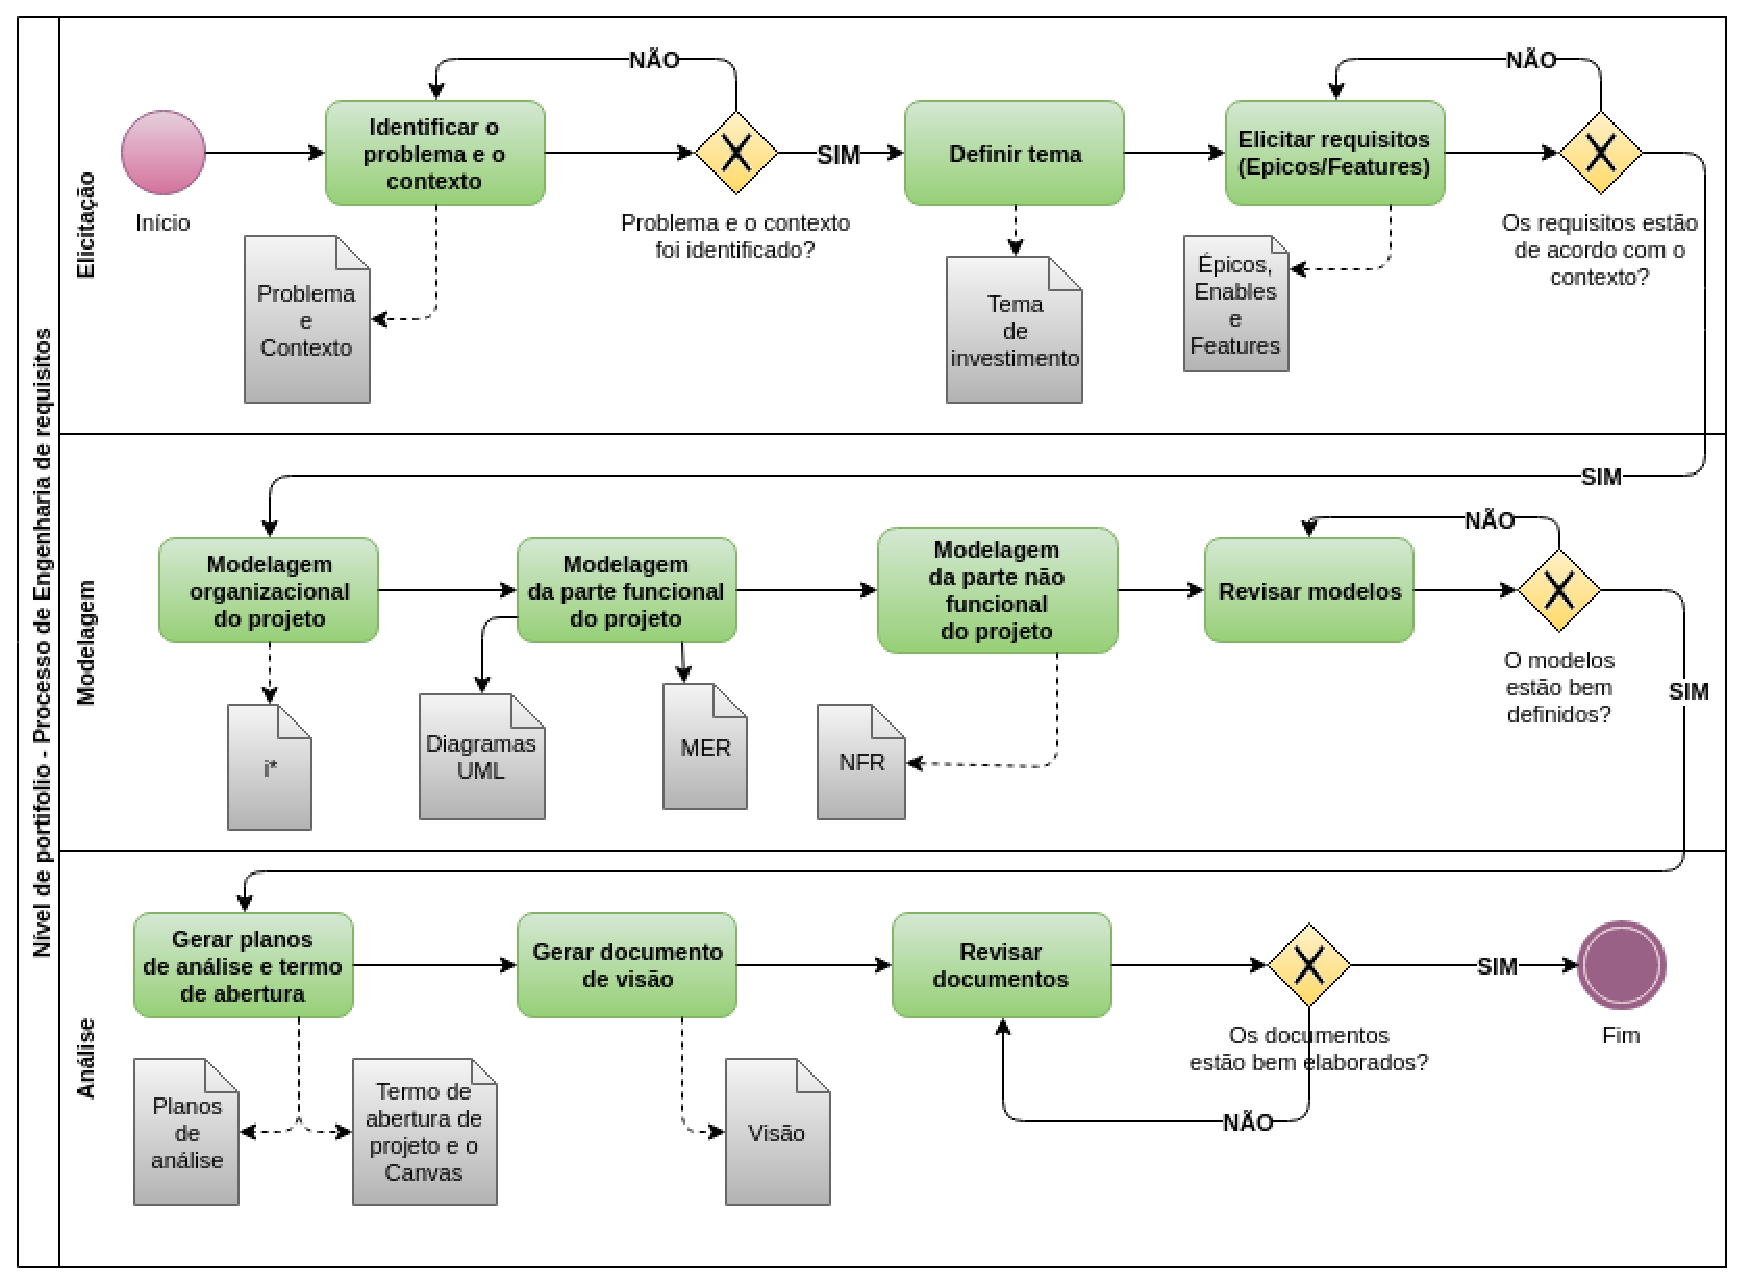
\includegraphics[keepaspectratio=true,scale=0.5]{figuras/requisitos.eps}
  \caption[Processo de engenharia de requisitos.]{Processo de engenharia de requisitos. Fonte: Autor}
	\label{fig:requisitos}
\end{figure}

\subsubsection{Atividades do processo de engenharia de requisitos (Elicitação)}

\begin{itemize}
  \item \textbf{Identificar o problema e o contexto}:
  \begin{itemize}
    \item \textbf{Descrição}: Nesta etapa, objetiva-se identificar o problema e o contexto na qual o software será aplicado.
    \item \textbf{Entradas}: N/A
    \item \textbf{Saídas}: Problema e contexto identificado.
  \end{itemize}
  \item \textbf{Definir tema}:
  \begin{itemize}
    \item \textbf{Descrição}: Nesta etapa, com o problema e o contexto bem definido será identificado o tema
      de investimento na qual o software será criado.
    \item \textbf{Entradas}: Problema e contexto
    \item \textbf{Saídas}: Tema de investimento
  \end{itemize}
  \item \textbf{Elicitar Requisitos}:
  \begin{itemize}
    \item \textbf{Descrição}: Nesta etapa, objetiva-se elicitar os requisitos através de técnicas de elicitação
      como brainstorm e prototipação. É nessa etapa que é identificado os Épicos (requisitos funcionais) e
      Enables (requisitos não funcionais) por meio do tema de investimento e os Épicos são separado em pedaços
      menores chamadas Features. Na rastreabilidade os épicos são identificados com a sigla ‘EP’, Enables com a
      sigla ‘EN’ e as Features com a sigla ‘FE’.
    \item \textbf{Entradas}: Tema de investimento
    \item \textbf{Saídas}: Épico, Enables e Features e sua rastreabilidade.
  \end{itemize}
\end{itemize}

\subsubsection{Atividades do processo de engenharia de requisitos (Modelagem)}

\begin{itemize}
  \item \textbf{Modelagem organizacional do projeto}:
  \begin{itemize}
    \item \textbf{Descrição}: Nesta etapa, objetiva-se criar um modelo organizacional em contexto com o uso do
      software.  Essa modelagem foi feito utilizando um framework chamado i* (i-estrela) originalmente proposto
      por Yu, trata da modelagem de contextos organizacionais tomando como base os relacionamentos de dependência
      entre os atores participantes. É dividido em Modelo SD (modelo de dependência estratégicas externa) e modelo
      SR (modelo de dependência estratégica interna)
    \item \textbf{Entradas}: Features
    \item \textbf{Saídas}: i* modelo SR e SD no documento de arquitetura do software.
  \end{itemize}
  \item \textbf{Modelagem da parte funcional do projeto}:
  \begin{itemize}
    \item \textbf{Descrição}: Nesta etapa, objetiva-se criar diagramas que auxilia na construção das
      funcionalidades do software por meio da modelagem UML como Diagrama de classe e criar a modelagem do
      banco de dados relacional por meio do Modelo Entidade Relacionamento (MER).
    \item \textbf{Entradas}: Features
    \item \textbf{Saídas}: Diagrama de classe e MER.
  \end{itemize}
  \item \textbf{Modelagem da parte não funcional do projeto}:
  \begin{itemize}
    \item \textbf{Descrição}: Nesta etapa, objetiva-se criar diagramas que auxilia a identificar requisitos não
      funcionais do software como metas a serem alcançadas por meio do framework NFR.
    \item \textbf{Entradas}: Enables
    \item \textbf{Saídas}: Framework NFR.
  \end{itemize}
  \item \textbf{Revisar modelos}:
  \begin{itemize}
    \item \textbf{Descrição}: Nesta etapa, objetiva-se revisar todos os diagramas em cada iteração do ciclo
      de desenvolvimento.
    \item \textbf{Entradas}: i*, NFR, MER e Diagrama de Classe
    \item \textbf{Saídas}: i*, NFR, MER e Diagrama de classe refinados
  \end{itemize}
\end{itemize}

\subsubsection{Atividades do processo de engenharia de requisitos (Análise)}

\begin{itemize}
  \item \textbf{Gerar planos de análise}:
  \begin{itemize}
    \item \textbf{Descrição}: Nesta etapa, objetiva-se criar todos os documentos relacionados ao gerenciamento do
      projeto, como por exemplo, documento de abertura do projeto, que terá um resumo dos documentos de gerenciamento
      como plano de gerenciamento de recursos humanos, comunicação, risco, medição e análise, configuração de
      software, aquisição e custos.
    \item \textbf{Entradas}: Modelo organizacional, funcional e não funcional
    \item \textbf{Saídas}: Planos de análise, Termo de abertura de projeto, Canvas.
  \end{itemize}
  \item \textbf{Gerar documento de visão}:
  \begin{itemize}
    \item \textbf{Descrição}: Nesta etapa, objetiva-se criar o documento de visão do produto
    \item \textbf{Entradas}: Requisitos, Planos de análise, Termo de abertura e Canvas
    \item \textbf{Saídas}: Documento de visão
  \end{itemize}
  \item \textbf{Revisar documentos}:
  \begin{itemize}
    \item \textbf{Descrição}: Nesta etapa, objetiva-se revisar os documentos criados anteriormente
    \item \textbf{Entradas}: Documento de visão, Planos de análise, Termo de abertura e Canvas
    \item \textbf{Saídas}: Documentos revisados e refinados
  \end{itemize}
\end{itemize}
